\documentclass[tikz,border=8pt]{standalone}
\usepackage{amsmath}\usepackage{pgfplots}
\pgfplotsset{compat=1.18}
\definecolor{ink}{HTML}{21352F}\definecolor{teal}{HTML}{087F7B}\definecolor{gold}{HTML}{C58B2A}\definecolor{rose}{HTML}{B65A62}\definecolor{blue}{HTML}{4B77A8}
\begin{document}
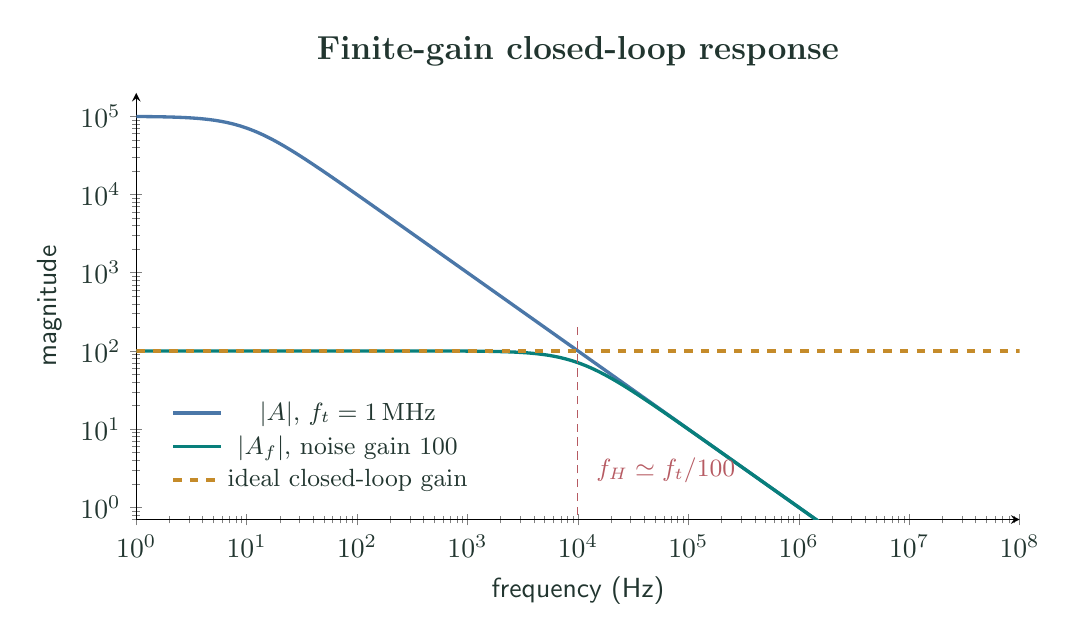
\begin{tikzpicture}[font=\sffamily,text=ink]
\begin{axis}[width=12.8cm,height=7cm,xmode=log,ymode=log,xmin=1,xmax=1e8,ymin=.7,ymax=2e5,axis lines=left,xlabel={frequency (Hz)},ylabel={magnitude},legend style={draw=none,fill=none,at={(.03,.04)},anchor=south west,font=\small},title={Finite-gain closed-loop response},title style={font=\bfseries\large}]
 \addplot[blue,very thick,domain=1:1e8,samples=300] {1e5/sqrt(1+(x/10)^2)};\addlegendentry{$|A|$, $f_t=1\,$MHz}
 \addplot[teal,very thick,domain=1:1e8,samples=300] {100/sqrt(1+(x/1e4)^2)};\addlegendentry{$|A_f|$, noise gain $100$}
 \addplot[gold,dashed,very thick,domain=1:1e8] {100};\addlegendentry{ideal closed-loop gain}
 \draw[rose,densely dashed] (axis cs:1e4,.8)--(axis cs:1e4,200);
 \node[rose,font=\small,anchor=west] at (axis cs:1.2e4,3) {$f_H\simeq f_t/100$};
\end{axis}
\end{tikzpicture}
\end{document}
